\chapter{Θεωρητικό Υπόβαθρο}
\label{ch:theoretical_background}

\section{Πλέγματα}
\begin{wrapfigure}{r}{0.25\textwidth}
    \centering
    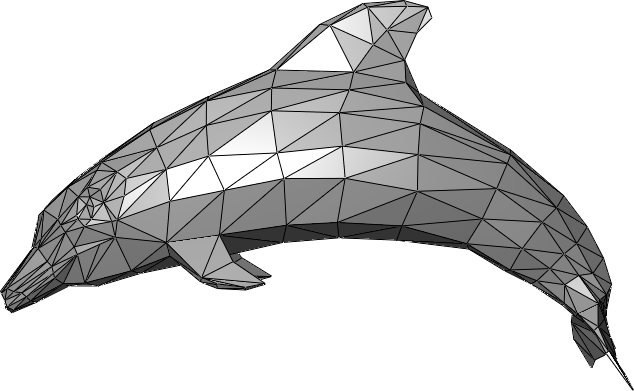
\includegraphics[width=0.25\textwidth]{Dolphin_triangle_mesh.png}
    \caption[Παράδειγμα Τριγωνικού Πλέγματος]{
        Παράδειγμα τριγωνικού πλέγματος που αναπαριστά ένα δελφίνι.
    }
    \label{fig:example_mesh}
\end{wrapfigure}
\label{sec:triangle_meshes}
Στην Υπολογιστική Γεωμετρία τα \textit{πλέγματα} αποτελούν την αναπαράσταση
μιας μεγαλύτερης γεωμετρικής περιοχής από μικρότερα διακριτά στοιχεία.
Τα πλέγματα χρησιμοποιούνται συνήθως για τον υπολογισμό λύσεων μερικών 
διαφορικών εξισώσεων, για την απόδοση γραφικών υπολογιστών, και για
ανάλυση γεωγραφικών και χαρτογραφικών δεδομένων.
Ένα πλέγμα χωρίζει τον χώρο σε μικρότερα στοιχεία (πολύγωνα ή πολύεδρα) όπου
μπορούν να λυθούν οι εξισώσεις, το οποίο στη συνέχεια προσεγγίζει τη λύση 
στο ευρύτερο πεδίο. 
Τα πλέγματα που αποτελούνται από πολύεδρα αντιπροσωπεύουν ρητά τόσο την 
επιφάνεια όσο και τον όγκο ενός αντικειμένου, ενώ τα πολυγωνικά 
πλέγματα αντιπροσωπεύουν μόνο την επιφάνεια (ο όγκος υπονοείται).
Για το πρόβλημα υπολογισμού της Ευκλείδειας απόστασης, ενδιαφερόμαστε 
μόνο για την εξωτερική επιφάνεια των αντικειμένων του τρισδιάστατου χώρου. 

Ένας τύπος πολυγωνικών πλεγμάτων είναι τα τριγωνικά πλέγματα 
(σχήμα \ref{fig:example_mesh}).
Αποτελούνται από ένα σύνολο τριγώνων στις τρεις διαστάσεις, 
τα οποία συνδέονται με τις κοινές τους ακμές ή κορυφές. 
Γεωμετρικά, ένα πλέγμα είναι μια τμηματικά επίπεδη επιφάνεια.
Η τελευταία ιδιότητα ισχύει πάντοτε για τα τριγωνικά πλέγματα.

Υπάρχουν διάφοροι τρόποι για την αποθήκευση ενός τριγωνικού πλέγματος 
στη μνήμη του υπολογιστή. 
Υπάρχουν επίσης μέθοδοι μετατροπής του ενός 
τρόπου αποθήκευσης σε έναν άλλο.
Ενδεικτικά αναφέρουμε την αποθήκευση με:
\begin{itemize}
    \item \textbf{Σετ τριγώνων}: 
    Το πλέγμα αναπαρίσταται απλά από τα τρίγωνα 
    του. 
    Δηλαδή αποθηκεύονται οι συντεταγμένες των κορυφών κάθε τριγώνου.
    \item \textbf{Σετ Τριγώνων με δείκτες}: 
    Το πλέγμα αναπαρίσταται από ένα σετ
    κόμβων και ένα σετ από τριπλέτες με δείκτες στους κόμβους.
    Η κάθε τριπλέτα αναπαριστά ένα τρίγωνο.
    \item \textbf{Λωρίδες Τριγώνων}: 
    Η αποθήκευση αυτή βασίζεται στο γεγονός ότι 
    δύο γειτονικά τρίγωνα μοιράζονται τη μία τους πλευρά. Αυτός 
    ο τρόπος χρησιμοποιείται για συμπίεση των πλεγμάτων.
    \item \textbf{Δομή Τρίγωνου-Γείτονα}: 
    Υποστηρίζει ερωτήματα γειτνίασης τριγώνων.
    \item \textbf{Δομή \tl{Winged-Edge}}: 
    Αποθηκεύει δεδομένα κόμβων, ακμών και όψεων.
    Επιτρέπει εύκολη διάβαση στο πλέγμα μεταξύ όψεων, ακμών και κορυφών.
\end{itemize} 
Για τους αλγορίθμους που περιγράφουμε παρακάτω αρκεί ο πρώτος τρόπος 
αναπαράστασης. 

Τέλος, για τις διάφορες εφαρμογές που χρησιμοποιούνται, τα πλέγματα 
χαρακτηρίζονται και από την ποιότητα τους. Οι πιο συνηθισμένες μετρικές 
ποιότητας είναι:
\begin{itemize}
    \item \textbf{Λοξότητα (\tl{Skewness})}: \\
    Η λοξότητα είναι ο λόγος της απόκλισης μεταξύ του βέλτιστου μεγέθους
    στοιχείου προς στο υπάρχον μέγεθος στοιχείου. 
    Το εύρος της λοξότητας είναι μεταξύ 0 (ιδανικό) έως 1 (χειρότερο).
    Τα πολύ λοξά στοιχεία δεν προτιμώνται λόγω της κακής ακρίβειας 
    που προκαλούν στις παρεμβαλλόμενες περιοχές.
    Ανάλογα με το στοιχείο (τρίγωνο, τετράπλευρο, τετράεδρο, 
    εξάεδρο κλπ) διαφοροποιείται μαθηματικός τύπος 
    για τον υπολογισμό της λοξότητας.

    \item \textbf{Ομαλότητα (\tl{Smoothness})}: \\
    Η αλλαγή στο μέγεθος των στοιχείων πρέπει να είναι ομαλή. 
    Συνήθως αποφεύγονται ξαφνικά άλματα στο μέγεθος των στοιχείων γιατί αυτό 
    μπορεί να προκαλέσει λανθασμένα αποτελέσματα σε κοντινούς κόμβους.
    
    \item \textbf{Αναλογία Διαστάσεων (\tl{Aspect Ratio})}: \\
    Εν συντομία, ο λόγος διαστάσεων είναι ο λόγος του μεγαλύτερου μήκους 
    ενός στοιχείου προς το μικρότερο μήκος. 
    Ο ιδανικός λόγος διαστάσεων είναι 1. 
    Όσο μικρότερος είναι, τόσο υψηλότερη είναι η ποιότητα ενός στοιχείου. 
    Η μέθοδος υπολογισμού ποικίλλει ανάλογα με τον τύπο κελιού.
\end{itemize}

Σε πραγματικές εφαρμογές, τα πλέγματα συνήθως σχεδιάζονται έτσι ώστε 
να μην παραβιάζουν σε μεγάλο βαθμό τις παραπάνω μετρικές ποιότητας.
Αυτή η παρατήρηση είναι χρήσιμη για τον σχεδιασμό της δομής δεδομένων 
που προτείνουμε.

\begin{figure}[h]
    \centering
    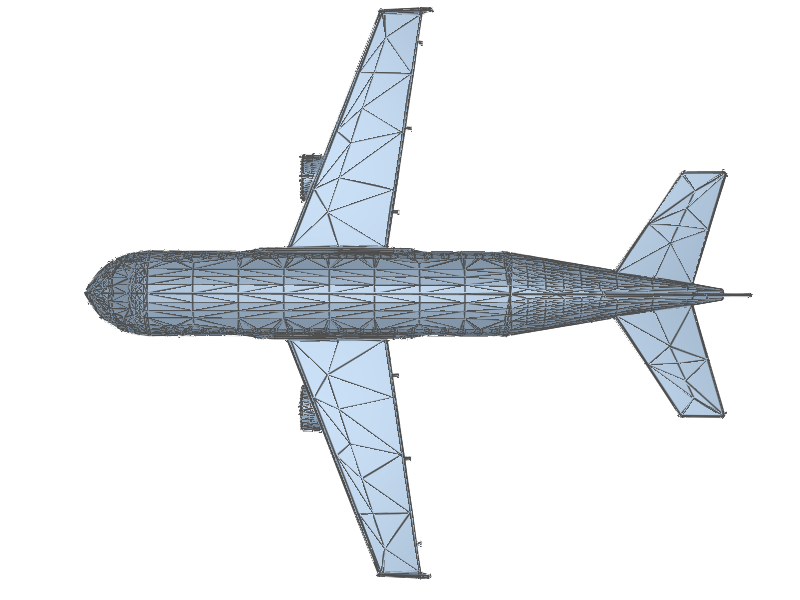
\includegraphics[width=0.45\textwidth]{airplane_bad_mesh.png}
    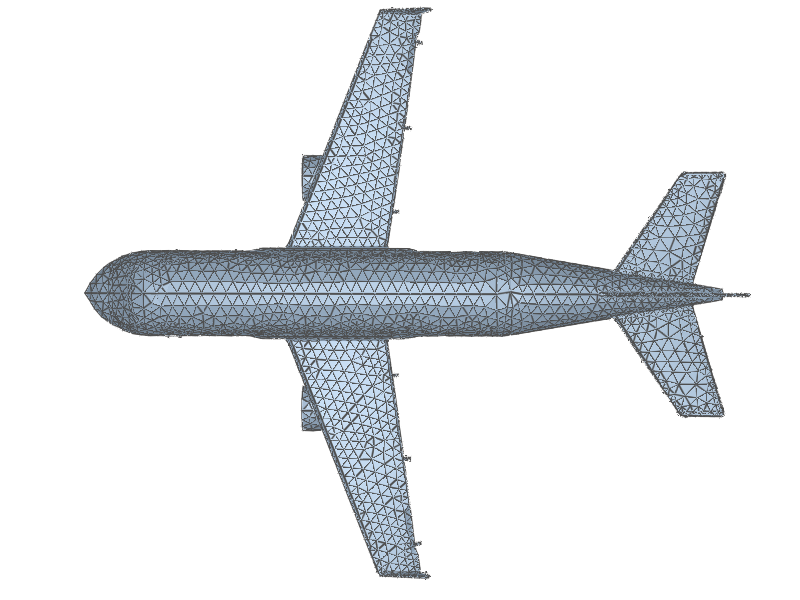
\includegraphics[width=0.45\textwidth]{airplane_good_mesh.png}
    \caption[Παράδειγμα Ποιότητας Πλεγμάτων]{
        Παράδειγμα Ποιότητας Πλεγμάτων - Και τα δύο πλέγματα 
        αναπαριστούν το ίδιο αεροπλάνο. Το δεξί πλέγμα είναι 
        καλύτερης ποιότητας από το αριστερό που φαίνεται να 
        παραβιάζει όλα τα κριτήρια ποιότητας που αναφέρθηκαν
        (\tl{skweness, smoothness, aspect ratio}). Και τα 
        δύο πλέγματα αποτελούνται από τον ίδιο αριθμό τριγώνων
        περίπου (γύρω στα $15000$ τρίγωνα).
    }
\end{figure}

\section{Οριοθετικοί Όγκοι}
\label{sec:bounding_volumes}
\textit{Οριοθετικός όγκος} (\textbf{\tl{bounding volume}}) ενός συνόλου 
από αντικείμενα του τρισδιάστατου χώρου ονομάζεται οποιοσδήποτε 
κλειστός όγκος που εξ' ολοκλήρου περικλείει τα αντικείμενα του συνόλου. 
Οι οριοθετικοί όγκοι χρησιμοποιούνται για να επιταχύνουν αλγορίθμους   
που εκτελούν γεωμετρικούς ελέγχους χρησιμοποιώντας απλούς όγκους 
που περικλείουν πολύπλοκα αντικείμενα.
Οι έλεγχοι σε οριοθετικούς όγκους είναι τυπικά πολύ ταχύτεροι από 
ελέγχους στο ίδιο το στοιχείο ή αντικείμενο που περικλείουν 
Σε πολλές περιπτώσεις, ένας έλεγχος αρκεί για να απορριφθούν ή 
να επιβεβαιωθούν πολλαπλοί έλεγχοι που θα απαιτούνταν για κάθε ένα 
από τα στοιχεία ξεχωριστά.

Οι οριοθετικοί όγκοι βρίσκουν ευρεία εφαρμογή στους παρακάτω τομείς:
\begin{itemize}
    \item \textbf{Ανίχνευση Ακτίνων (\tl{Ray Tracing})}:\\
    Oι οριοθετικοί όγκοι χρησιμοποιούνται σε ελέγχους τομής ακτίνων 
    με αντικείμενα και σε πολλούς αλγόριθμους απόδοσης γραφικών.
    Για παράδειγμα, εάν η ακτίνα ή το οπτικό πεδίο της κάμερας
    δεν τέμνει τον οριοθετικό όγκο, τότε δεν μπορεί να τέμνει ούτε 
    το αντικείμενο που περιέχεται μέσα. Έτσι αποφεύγονται οι 
    αντίστοιχοι έλεγχοι, οι οποίοι κοστίζουν υπολογιστικά.
    Όμοια, εάν το οπτικό πεδίο της κάμερας περιέχει εξ ολοκλήρου 
    τον οριοθετικό όγκο, το αντικείμενο, δηλαδή τα στοιχεία από τα
    οποία αποτελείται θα απεικονιστούν στην 
    οθόνη χωρίς περισσότερους ελέγχους. 
    
    \item \textbf{Ανίχνευση Σύγκρουσης (\tl{Collision Detection})}:\\
    Όμοια με πριν, όταν δύο οριοθετικοί όγκοι δε συγκρούονται/τέμνονται, 
    τότε ούτε και τα αντικείμενα που περικλείουν δεν μπορούν να συγκρούονται.
\end{itemize}

Για τη δημιουργία οριοθετικών όγκων σύνθετων αντικειμένων, συνήθως 
χρησιμοποιούνται \textit{Ιεραρχίες Οριοθετικών Όγκων} (βλ. \ref{sec:bvh}).
Δηλαδή, δενδρικές δομές δεδομένων όπου η βασική ιδέα κατασκευής τους 
είναι η ρίζα να περικλείει ολόκληρο το αντικείμενο ενώ τα φύλλα 
ένα μικρό υποσύνολο του.

Η επιλογή του τύπου οριοθετικού όγκου για μια δεδομένη εφαρμογή 
καθορίζεται από διάφορους παράγοντες. Τέτοιοι είναι το κόστος υπολογισμού
ενός οριοθετικού όγκου για ένα αντικείμενο, το κόστος της ενημέρωσης
του σε εφαρμογές στις οποίες τα αντικείμενα μπορούν να μετακινηθούν 
ή να αλλάξουν σχήμα, το κόστος ανίχνευσης σύγκρουσης 
ή υπολογισμού απόστασης και η επιθυμητή 
ακρίβεια για ελέγχους σύγκρουσης ή απόστασης. Η ακρίβεια αυτή σχετίζεται 
με τον όγκο του \textit{κενού χώρου} που περικλείεται από τον οριοθετικό όγκο
όμως δε σχετίζεται με το οριοθετημένο αντικείμενο. Τυπικά, ισχύει ο εξής
συμβιβασμός: οι πιο εκλεπτυσμένοι οριοθετικοί όγκοι περικλείουν γενικά 
λιγότερο κενό χώρο, αλλά είναι πιο ακριβοί υπολογιστικά. 

Οι πιο συνηθισμένοι τύποι οριοθετικών όγκων είναι:
\begin{itemize}
    \item Η \textbf{Οριοθετική Σφαίρα (\tl{Bounding Sphere})}, 
    η οποία είναι μια σφαίρα που περικλείει το αντικείμενο. 
    Αναπαρίσταται από το κέντρο και την ακτίνα της και 
    επιτρέπει πολύ γρήγορους ελέγχους σύγκρουσης και 
    υπολογισμού απόστασης. 
    Δύο σφαίρες τέμνονται όταν η απόσταση μεταξύ των κέντρων τους 
    δεν υπερβαίνει το άθροισμα των ακτίνων τους.

    \item Ο \textbf{Οριοθετικός Κύλινδρος (\tl{Bounding Cylinder})}, 
    είναι ένας κύλινδρος που περικλείει το αντικείμενο. 
    Στις περισσότερες εφαρμογές ο άξονας του κυλίνδρου είναι 
    ευθυγραμμισμένος με την κατακόρυφη διεύθυνση της σκηνής.
    Οι κύλινδροι είναι κατάλληλοι για τρισδιάστατα αντικείμενα 
    που μπορούν να περιστρέφονται μόνο γύρω από έναν κατακόρυφο άξονα 
    αλλά όχι γύρω από άλλους άξονες, και κατά τα άλλα η κίνηση τους 
    να είναι μόνο μεταφορική. 
    Δύο κύλινδροι ευθυγραμμισμένοι με κατακόρυφο άξονα τέμνονται όταν, 
    ταυτόχρονα, τέμνονται οι προβολές τους στον κατακόρυφο άξονα (που είναι 
    ευθύγραμμα τμήματα), καθώς και οι προβολές τους 
    στο οριζόντιο επίπεδο (που είναι κύκλοι). 
    Οι δύο συνθήκες είναι εύκολο να ελεγχθούν. 
    Στα βιντεοπαιχνίδια, οι οριοθετικοί κύλινδροι χρησιμοποιούνται 
    συχνά ως οριοθετικοί όγκοι για χαρακτήρες που στέκονται όρθια.

    \item Το \textbf{Οριοθετικό Πλαίσιο (\tl{Bounding Box})}, είναι ένα 
    ορθογώνιο παραλληλεπίπεδο που περικλείει το αντικείμενο. 
    Στις προσομοιώσεις όπου η σκηνή αλλάζει δυναμικά, τα οριοθετικά πλαίσια
    προτιμώνται από άλλα σχήματα οριοθετικών όγκων (σφαίρες ή κυλίνδρους) 
    για αντικείμενα που έχουν χονδρικά κυβοειδές σχήμα
    όταν ο έλεγχος σύγκρουσης πρέπει να είναι αρκετά ακριβής.
    Το όφελος είναι προφανές, για παράδειγμα, για αντικείμενα 
    που ακουμπούν πάνω σε άλλα, όπως ένα αυτοκίνητο που ακουμπά 
    στο έδαφος: μια οριοθετική σφαίρα θα έδειχνε πως το αυτοκίνητο 
    πιθανώς να τέμνεται με το έδαφος, το οποίο στη συνέχεια θα έπρεπε 
    να απορριφθεί από μια πιο ακριβή υπολογιστικά δοκιμή του πραγματικού 
    μοντέλου του αυτοκινήτου. Ένα οριοθετικό πλαίσιο δείχνει αμέσως 
    ότι το αυτοκίνητο δεν τέμνεται με το έδαφος, 
    εξοικονομώντας έτσι την κοστοβόρα δοκιμή.

    Στη γενική περίπτωση, 
    ένα αυθαίρετο οριοθετικό πλαίσιο ονομάζεται και \textbf{Προσανατολισμένο 
    Οριοθετικό Πλαίσιο (\tl{Oriented Bounding Box})} \textbf{\tl{OBB}} 
    ή \textbf{\tl{OOBB}} όταν χρησιμοποιείται το τοπικό σύστημα 
    συντεταγμένων ενός αντικειμένου.
    Σε πολλές εφαρμογές το οριοθετικό πλαίσιο είναι ευθυγραμμισμένο με τους 
    άξονες του συστήματος συντεταγμένων και ονομάζεται \textbf{Οριοθετικό 
    Πλαίσιο Ευθυγραμμισμένο με τους Άξονες (\tl{Axis-Aligned Bounding Box})}
    ή \textbf{\tl{AABB}}. 
    Τα \tl{AABB} είναι πιο απλά και αποδοτικά στην ανίχνευση 
    σύγκρουσης μεταξύ τους από τα \tl{OBB}, αλλά έχουν το μειονέκτημα ότι 
    όταν το μοντέλο  περιστρέφεται δεν μπορούν απλώς να περιστραφούν με αυτό, 
    αλλά πρέπει να υπολογιστούν εκ νέου. 

    Στην περίπτωση των δύο διαστάσεων, χρησιμοποιείται το 
    \textbf{Ελάχιστο Οριοθετικό Παραλληλόγραμμο (\tl{Minimum Bounding Rectangle})}
    ή \tl{\textbf{MBR}}. Το \tl{MBR} είναι ειδική περίπτωση του \tl{AABB} στο 
    επίπεδο και χρησιμοποιείται συχνά για να περικλείει γεωγραφικά (ή γεωχωρικά)
    δεδομένα.

    \item H \textbf{Οριοθετική Κάψουλα (\tl{Bounding Capsule})}, 
    η οποία προκύπτει από τον συνολικό όγκο που περικλείει μια σφαίρα 
    καθώς κινείται πάνω σε ένα ευθύγραμμο τμήμα (\tl{swept sphere}). 
    Ο όγκος που προκύπτει αποτελείται από έναν κύλινδρο και δύο 
    ημισφαίρια στα άκρα του.
    Μπορούν να αναπαρασταθούν από το ευθύγραμμο τμήμα και το μήκος 
    της ακτίνας της σφαίρας.
    Έχει χαρακτηριστικά παρόμοια με έναν κύλινδρο, αλλά είναι πιο εύκολη 
    στη χρήση, επειδή ο έλεγχος σύγκρουσης είναι απλούστερος.
    Για παράδειγμα, δύο κάψουλες τέμνονται εάν η απόσταση μεταξύ των τμημάτων
    που τις ορίζουν είναι μικρότερη από το άθροισμα των ακτίνων τους.
    Αυτό ισχύει για τις αυθαίρετα προσανατολισμένες κάψουλες, γι' 
    αυτό είναι πιο ελκυστικές από τους κυλίνδρους στην πράξη.
\end{itemize}

Στα πλαίσια αυτής της εργασίας, θα χρησιμοποιηθούν τα \tl{AABB}.

\section{Ιεραρχίες Οριοθετικών Όγκων}
\label{sec:bvh}
H \textit{Ιεραρχία Οριοθετικών Όγκων} (\tl{\textbf{Bounding Volume Hierarchy}}
ή \tl{\textbf{BVH}}) είναι μια δενδρική δομή που αποθηκεύει και οργανώνει 
γεωμετρικά (ή χωρικά) στοιχεία (\tl{elements}). 
Τέτοια είναι τα πολύτοπα, 
τα πολύεδρα, παραμετρικές καμπύλες ή επιφάνειες και άλλα. 
Κάθε κόμβος του δένδρου αναπαρίσταται από τον οριοθετικό όγκο του
υποσυνόλου των στοιχείων που αποθηκεύει. 
Ο όγκος αυτός προκύπτει από τη συγχώνευση των οριοθετικών όγκων των παιδιών 
του κόμβου.
Με αυτό τον αναδρομικό τρόπο, οργανώνεται το σύνολο των στοιχείων του 
δένδρου από τα φύλλα έως τη ρίζα.
Συνεπώς, η ρίζα του δένδρου αναπαρίσταται από τον οριοθετικό όγκο που περικλείει 
όλα τα στοιχεία του δένδρου, ενώ τα φύλλα αναπαρίστανται από τους οριοθετικούς
όγκους του κάθε στοιχείου ξεχωριστά (βλ. Σχήμα \ref{fig:bvh_example_2d}).

\begin{figure}[h]
    \centering
    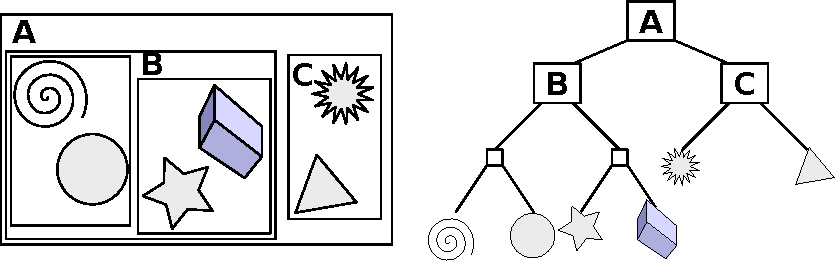
\includegraphics[width=0.8\textwidth]{bvh_example.pdf}
    \caption[Οπτικοποίηση μιας Ιεραρχίας Οριοθετικών Όγκων]{
        Παράδειγμα μιας Ιεραρχίας Οριοθετικών Όγκων στις δύο 
        διαστάσεις που χρησιμοποιεί ορθογώνια παραλληλόγραμμα 
        για οριοθετικούς όγκους.
        Αριστερά απεικονίζονται τα αντικείμενα και τα οριοθετικά 
        πλαίσια που περικλείουν τα αντικείμενα. Δεξιά απεικονίζεται 
        η ιεραρχία σε μορφή δέντρου.
        }
    \label{fig:bvh_example_2d}
\end{figure}

Γενικά, η ενθυλάκωση αντικειμένων μέσα σε οριοθετικούς όγκους επιταχύνει 
πολλές γεωμετρικές πράξεις πχ. \tl{collision detection}, \tl{ray tracing},
κλπ όπως έγινε φανερό στο \ref{sec:bounding_volumes},
παρ' όλα αυτά δε μειώνει τον αριθμό των ελέγχων που απαιτούνται.
Δηλαδή η υπολογιστική πολυπλοκότητα των αλγορίθμων παραμένει ίδια
(βλ. \ref{sec:exhaustive_search} για ένα παράδειγμα τέτοιου αλγορίθμου). 
Με την οργάνωση των αντικειμένων σε ιεραρχίες 
οριοθετικών όγκων, ωστόσο, η υπολογιστική πολυπλοκότητα (δηλαδή το πλήθος 
των ελέγχων που εκτελούνται) μπορεί να μειωθεί 
σε λογαριθμική σε σχέση με το πλήθος των αντικειμένων.
Σε μια τέτοια ιεραρχία τα αντικείμενα ενός κόμβου δε χρειάζεται 
να εξετασθούν αν το αποτέλεσμα του ελέγχου μπορεί να εξακριβωθεί 
από κάποιον πρόγονό του.
Αυτή η τεχνική ονομάζεται κλάδεμα του δέντρου (\tl{tree pruning}).

Για τη σχεδίαση ιεραρχιών οριοθετικών όγκων υπάρχουν πολλές επιλογές. 
\begin{itemize}
    \item Η \textit{επιλογή του οριοθετικού όγκου} 
    που θα χρησιμοποιείται από την ιεραρχία παίζει σημαντικό λόγο. 
    Η επιλογή καθορίζεται από μια σύμβαση μεταξύ δύο στόχων: 
    Από τη μία πλευρά, θα θέλαμε να χρησιμοποιήσουμε
    οριοθετικούς όγκους που έχουν πολύ απλό σχήμα γιατί η αποθήκευση τους 
    στη μνήνη είναι μικρή και οι διάφοροι γεωμετρικοί έλεγχοι είναι 
    γρήγοροι.
    Από την άλλη πλευρά, θα θέλαμε να έχουμε οριοθετικούς όγκους που να
    περικλείουν πολύ στενά τα αντικείμενα.
    Ο πιο κοινός τύπος οριοθετικού όγκου που χρησιμοποιείται είναι τα
    \tl{AABB}.
    
    \item Η \textit{τεχνική κατασκευής του δένδρου} αποτελεί επίσης 
    σχεδιαστική επιλογή.
    Υπάρχουν τρεις κύριες κατηγορίες αλγορίθμων κατασκευής δένδρων: 
    \begin{itemize}
        \item Οι \textit{από πάνω προς τα κάτω (\tl{top-down})}, οι 
        οποίοι λειτουργούν με διαμερισμό του συνόλου εισόδου σε δύο (ή περισσότερα)
        υποσύνολα, οριοθετώντας τα στον επιλεγμένο 
        οριοθετικό όγκο και, στη συνέχεια, επαναλαμβάνουν την ίδια 
        διαδικασία αναδρομικά έως ότου κάθε υποσύνολο να αποτελείται 
        από ένα μόνο στοιχείο (δηλαδή η διαδικασία τερματίζει 
        όταν φτάσει στα φύλλα του δέντρου).
        
        \item Οι \textit{από κάτω προς τα πάνω (\tl{bottom-up})}, οι
        οποίοι ξεκινούν με το σύνολο των στοιχείων που αποθηκεύονται 
        στα φύλλα του δέντρου και στη συνέχεια ομαδοποιούν δύο (ή περισσότερα) 
        από αυτά για να σχηματίσουν έναν νέο εσωτερικό κόμβο.
        Η διαδικασία συνεχίζεται με τον ίδιο τρόπο έως ότου όλα 
        τα στοιχεία ομαδοποιηθούν σε έναν μόνο κόμβο (τη ρίζα του δέντρου).
        Οι μέθοδοι από κάτω προς τα πάνω είναι πιο δύσκολοι στην υλοποίηση, 
        αλλά είναι πιθανό να παράγουν καλύτερης ποιότητας δέντρα γενικά.
        Ένας ευρέως διαδεδομένος τρόπος για ομαδοποίηση των δεδομένων από κάτω 
        προς τα πάνω είναι η χρήση \textit{καμπυλών πλήρωσης χώρου
        (\tl{space filling curves})} \cite{gu2013efficient} \cite{tero2012construct}. 
        Τα στοιχεία ταξινομούνται αρχικά με βάση την καμπύλη και 
        ομαδοποιούνται σύμφωνα με την ακολουθία που προκύπτει.
        
        \item Οι \textit{μέθοδοι με εισαγωγή (\tl{insertion methods})}, οι 
        οποίοι κατασκευάζουν το δέντρο εισάγοντας ένα στοιχείο τη φορά, 
        ξεκινώντας από ένα κενό δέντρο. 
        Η θέση που τοποθετείται ένα νέο στοιχείο επιλέγεται έτσι ώστε 
        το δέντρο να μεγαλώσει όσο το δυνατόν λιγότερο, σύμφωνα με κάποια 
        μετρική κόστους.
        Οι μέθοδοι με εισαγωγή θεωρούνται \tl{on-line} μέθοδοι δεδομένου ότι
        δεν απαιτούν να είναι διαθέσιμα όλα τα στοιχεία πριν από την έναρξη
        της κατασκευής και επομένως επιτρέπουν την εκτέλεση ενημερώσεων 
        (\tl{updates}) κατά το χρόνο εκτέλεσης.
        Οι άλλες δύο κατηγορίες που αναφέρθηκαν θεωρούνται \tl{off-line} 
        μέθοδοι καθώς και οι δύο απαιτούν να είναι διαθέσιμα όλα τα 
        στοιχεία πριν από την έναρξη της κατασκευής. 

        Η εισαγωγή στοιχείων στο \tl{BVH} συνήθως καταλήγει σε δέντρα με 
        χειρότερη επίδοση στα ερωτήματα σε σχέση με μια πλήρη ανακατασκευή
        από την αρχή. Οι λύσεις που προτείνονται είναι είτε η ασύγχρονη 
        ανακατασκευή του δέντρου, είτε η ανακατασκευή όταν ανιχνευθεί 
        σημαντική αλλαγή (πχ υπάρχει μεγάλη επικάλυψη κοντά στα φύλλα, 
        ή ο αριθμός των προσθαφαιρέσεων στοιχείων ξεπεράσει κάποιο 
        κατώφλι, ή άλλες πιο εκλεπτυσμένες ευρετικές μεθόδους).
    \end{itemize}
    
    \item Ο \textit{βαθμός} (αριθμός των παιδιών των κόμβων) του 
    δένδρου. 
    Ένα δέντρο χαμηλού βαθμού θα έχει μεγαλύτερο ύψος. 
    Αυτό αυξάνει τον χρόνο διάσχισης από τη ρίζα έως τα φύλλα.
    Από την άλλη πλευρά, λιγότεροι υπολογισμοί πρέπει να δαπανηθούν
    σε κάθε κόμβο που επισκέπτεται ο αλγόριθμος για να ελέγξει ποια 
    παιδιά θα επισκεφθεί και με ποια σειρά. 
    Το αντίθετο ισχύει για ένα δέντρο υψηλού βαθμού, δηλαδή αν και το δέντρο
    θα είναι μικρότερου ύψους, δαπανάται περισσότερη δουλειά σε κάθε κόμβο.
    Στην πράξη, τα δυαδικά δέντρα (βαθμός $ = 2$) είναι μακράν τα πιο κοινά. Ένας από τους κύριους λόγους είναι ότι τα δυαδικά δέντρα είναι πιο εύκολο να κατασκευαστούν.
    
    \item \textit{Η μέθοδος διάσχισης} του δένδρου για την απάντηση 
    γεωμετρικών ερωτημάτων. Όταν θα πρέπει να γίνει επίσκεψη σε 
    περισσότερα από ένα απ'ο τα παιδιά ενός κόμβου, 
    η σειρά με την οποία αυτά θα ελεγχθούν 
    δεν επηρεάζει την ορθότητα του αλγορίθμου, όμως έχει αντίκτυπο 
    στην επίδοση του.
\end{itemize}

Τέλος, αναφέρουμε κάποιες επιθυμητές ιδιότητες \cite{ericson2004real} 
μιας Ιεραρχίας Οριοθετικών Όγκων οι οποίες πρέπει να ληφθούν υπόψη 
κατά τον σχεδιασμό της για τις διάφορες εφαρμογές:
\begin{itemize}
    \item Τα στοιχεία που περιλαμβάνει οποιοδήποτε υπο-δέντρο 
    θα πρέπει να είναι κοντά το ένα στο άλλο (χωρικά). 
    Όσο πιο χαμηλά στο δέντρο, τόσο πιο κοντά θα πρέπει να 
    βρίσκονται τα αντικείμενα.
    \item Ο όγκος της επικάλυψης των αδελφικών κόμβων πρέπει να είναι ελάχιστος
    \item Κάθε κόμβος του δέντρου πρέπει να έχει τον ελάχιστο δυνατό όγκο.
    \item Το άθροισμα όλων των οριοθετικών όγκων πρέπει να είναι ελάχιστο.
    \item Θα πρέπει να δοθεί μεγαλύτερη προσοχή στους κόμβους κοντά στη 
    ρίζα του \tl{BVH}. 
    Το κλάδεμα ενός κόμβου κοντά στη ρίζα του δέντρου αφαιρεί περισσότερα αντικείμενα
    από περαιτέρω εξέταση.
    \item Το \tl{BVH} θα πρέπει να είναι όσο πιο ισορροπημένο γίνεται. 
    Η εξισορρόπηση επιτρέπει να κλαδευτεί όσο το δυνατόν μεγαλύτερο μέρος 
    του \tl{BVH} όποτε δε διασχίζεται ένα κλαδί.
\end{itemize}
